\documentclass[8pt]{beamer}

\mode<presentation> {
\usetheme{Madrid}
\setbeamertemplate{footline}[page number]
}

\usepackage{graphicx} % Allows including images
\usepackage{booktabs} % Allows the use of \toprule, \midrule and \bottomrule in tables
\usepackage{tabularx}  % for 'tabularx' environment and 'X' column type
\usepackage{ragged2e}  % for '\RaggedRight' macro (allows hyphenation)
\usepackage{grffile}
\newcolumntype{Y}{>{\RaggedRight\arraybackslash}X} 

\usepackage{amsfonts}
%\usepackage{tikz}
%\def\checkmark{\tikz\fill[scale=0.4](0,.35) -- (.25,0) -- (1,.7) -- (.25,.15) -- cycle;} 


\setcounter{figure}{0}

\title[Energy Efficient Vehicle Control]{Real World Optimization of Energy Efficient Vehicle Control}
\subtitle[Current State]{Current State}
\author{Bastian Lang} % Your name
\institute[BRSU] % Your institution as it will appear on the bottom of every slide, may be shorthand to save space
{
Bonn-Rhein-Sieg University of Applied Science \\ % Your institution for the title page
}
\date{\today} 
\titlegraphic{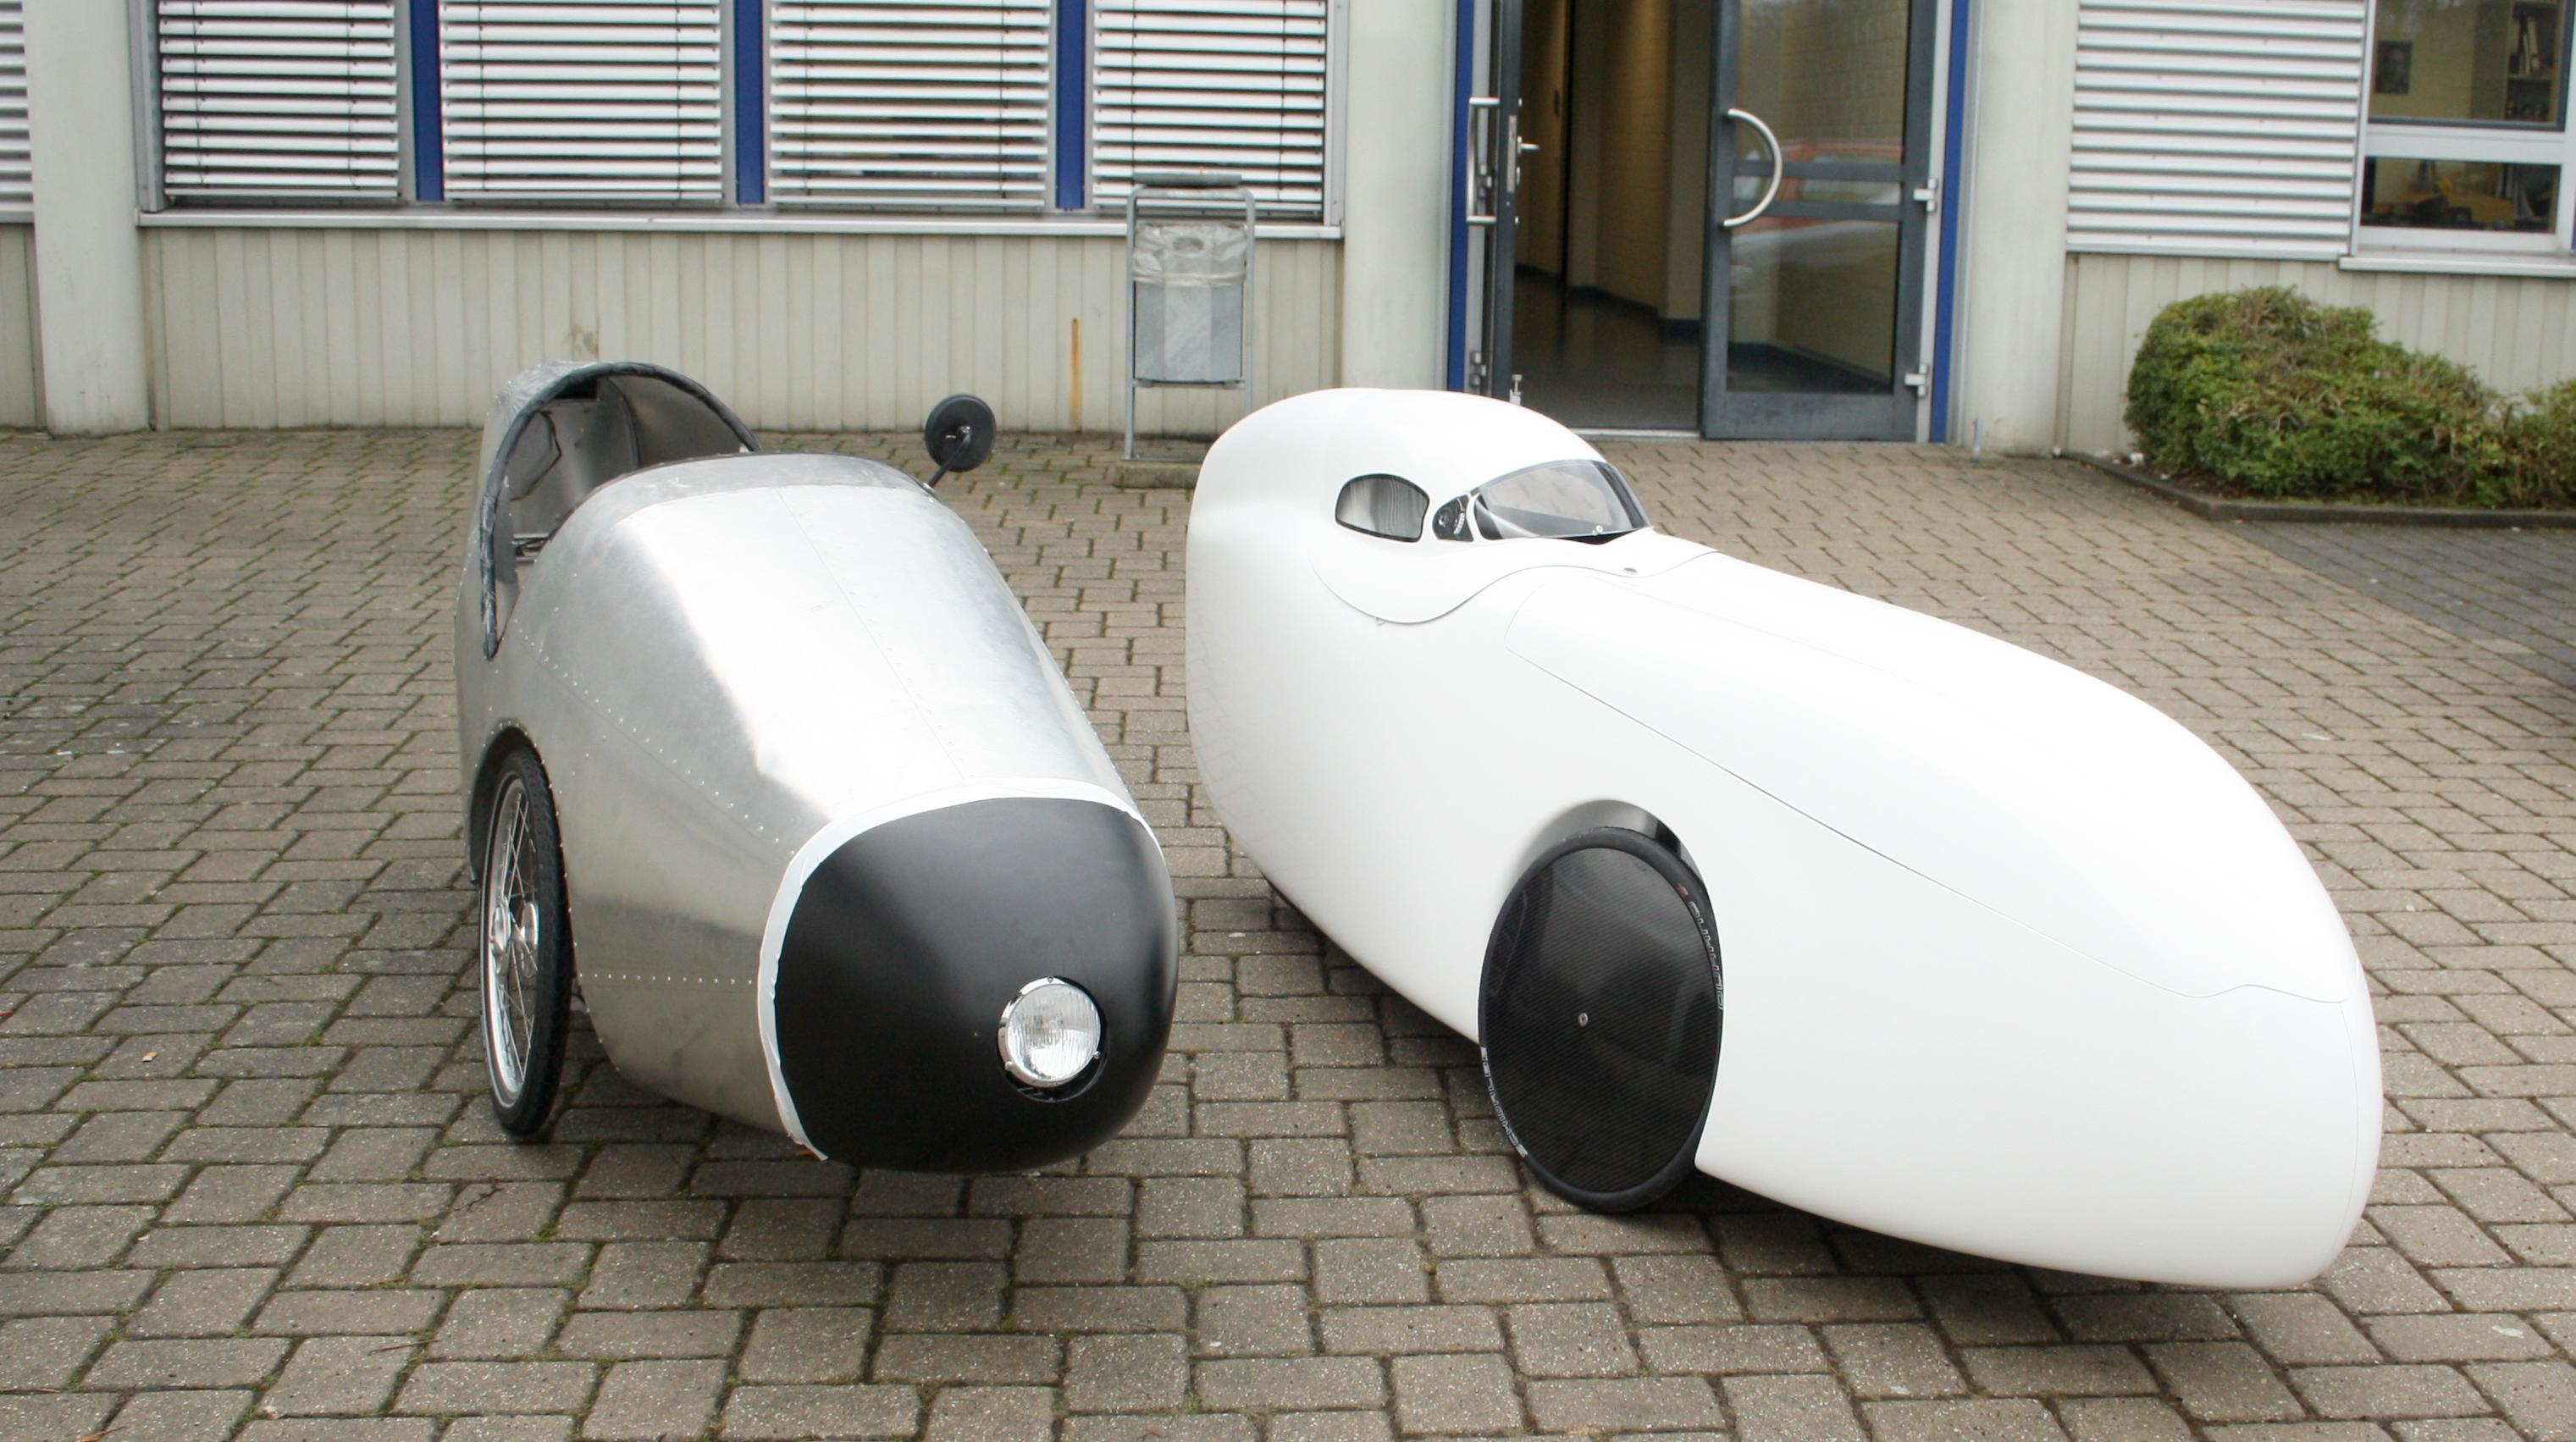
\includegraphics[width=6cm]{images/stella}}
\begin{document}

\listoffigures

\begin{frame}
	\titlepage
\end{frame}

\AtBeginSection[]{
	\begin{frame}
		\frametitle{Content}
		\tableofcontents[currentsection, hideothersubsections]
	\end{frame}
}
\begin{frame}
	\frametitle{Content}
	\tableofcontents[hideallsubsections]
\end{frame}

\section{Project Description}
\begin{frame}
	\frametitle{Project Description}
	\framesubtitle{Project Description}
	\begin{block}{What is the project about?}
		\pause
		Creating Energy Efficient Vehicle Controller  
	\end{block}	
	\pause	
	\begin{block}{What ML technologies are being used?}
		\pause
		ANNs evolved using NEAT
	\end{block}
	\pause
	\begin{block}{What is the project based on?}
		\pause		
		Paper showing ANNs can compete with state-of-the-art approaches (cite paper)
	\end{block}
\end{frame}

\begin{frame}
	\frametitle{Project Description}
	\framesubtitle{Task Overview}
	\pause
	\begin{block}{Minimum}
	\pause
	\begin{itemize}[<+->]
		\item Evolve Energy Efficient Controller with Simple Model
		\item Evaluate in Reality 
		\item Compare Simulation vs Reality
	\end{itemize}
	\end{block}	
	\pause
	
	\begin{block}{Expected}
	\pause
	\begin{itemize}[<+->]
		\item Create Data Driven Model 
		\item Evolve Energy Efficient Controller with DD Model
		\item Evaluate in Reality
		\item Compare Solutions		
	\end{itemize}
	\end{block}	
	\pause
	
	\begin{block}{Maximum}
	\pause
	\begin{itemize}[<+->]
		\item Use Multi-Objective Approach (i.e. Surrogate Modelling)
	\end{itemize}
	\end{block}
	
\end{frame}

\section{The Simple Model}
\begin{frame}
	\frametitle{Simple Vehicle Model}
	\begin{block}{Time Based Model}	
	\[
	\frac{ds}{dt} = \left(
			\begin{array}{ll}
			t' \\
			x' \\
			v' \\
			W'
			\end{array}
		\right)
		= \left(
			\begin{array}{ll}
			1 \\
			v \\
			\frac{F(x,v)}{m} \\
			F_u * v
			\end{array}
		\right)
	\]
	
	Where\\
	\begin{itemize}
		\item $F_U$: Force at wheel due to control command
		\item $F(x,v)$: $F_U$ - some drag
	\end{itemize}
	\end{block}

\end{frame}

\begin{frame}
	\frametitle{Simple Vehicle Model}
	Visualizations of Simulations
\end{frame}

\section{NEAT with the Simple Model}
\begin{frame}
	\frametitle{NEAT with the Simple Model}
	\framesubtitle{Data}
	\begin{block}{Tracks Used}
		\begin{itemize}
			\item 35
			\item cross validation
		\end{itemize}
	\end{block}
	\begin{block}{NEAT Parameters}
		\begin{itemize}
		
		
			\item population
			\item speciation kmeans
			\item maximum generations
			\item nr of runs
			\item topology
		\end{itemize}
	\end{block}
\end{frame}

\begin{frame}
	\frametitle{NEAT with the Simple Model}
	\framesubtitle{Results}
	\begin{itemize}
		\item Average Best Fitness
		\item Average Nr Generations
	\end{itemize}
\end{frame}

\begin{frame}
	\frametitle{NEAT with the Simple Model}
	\framesubtitle{Simulations}
\end{frame}

\section{Control Program for Velomobile}
\begin{frame}
	\frametitle{Control Program}
	TODO: diagram multi-threading
\end{frame}

\subsection{Control Program(s)}
\begin{frame}
	\frametitle{The Task}
\end{frame}
\subsection{Problems}
\begin{frame}
	\frametitle{The Task}
\end{frame}

\section{Open Tasks}
\begin{frame}
	\frametitle{The Task}
\end{frame}


\end{document} 